%&latex
\documentclass[a4paper]{article}

\frenchspacing

\usepackage[cp1250]{inputenc}
\usepackage[czech]{babel}

\usepackage{a4wide}
\usepackage{amsmath, amsthm, amssymb, amsfonts}
\usepackage[mathcal]{eucal}
\usepackage{graphicx}
\usepackage{url}
\usepackage{color}
\usepackage{wrapfig}
\usepackage{capt-of}
\usepackage{float}



% sirka a vyska textu nastavena jako papir, vsechny okraje vynulovany a pridano 20pt na kazdou stranu
% horizontalni rozmery
\setlength{\textwidth}{\paperwidth}
\addtolength{\textwidth}{-40pt}
\addtolength{\hoffset}{-1in}
\addtolength{\hoffset}{20pt}
\setlength{\oddsidemargin}{0in}
\setlength{\marginparsep}{0in}
% vertikalni rozmery
\setlength{\textheight}{\paperheight}
\addtolength{\textheight}{-60pt}
\addtolength{\voffset}{-1in}
\addtolength{\voffset}{20pt}
\setlength{\topmargin}{0in}
\setlength{\headheight}{0in}
\setlength{\headsep}{0in}


%Obrazek na miste
%pouziti
%%\obrazeknahore{adresa}{popisek}{label}
\long\def\obrazeknahore#1#2#3 {

\begin{figure}[t]
    \centering
    \includegraphics[width=0.8\textwidth]{#1}
    
    \caption{#2}
    \label{#3}
    
\end{figure}

}


%==========================================
%PEKELNA MAKRA NA ZAROVNANI OBRAZKU DOPRAVA

\makeatletter


%tohle je makro, ktere mi dovoluje obtekani i u kratkych environmentu
%ABSOLUTNE nechapu, jak to funguje, ale funguje to
%viz http://tex.stackexchange.com/questions/26078/ 
\def\odrovnej{\@@par
\ifnum\@@parshape=\z@ \let\WF@pspars\@empty \fi % reset `parshape'
\global\advance\c@WF@wrappedlines-\prevgraf \prevgraf\z@
\ifnum\c@WF@wrappedlines<\tw@ \WF@finale \fi}

\makeatother



%---
%makro, co da obrazek doprava a ostatni text ho obteka
%(bez toho predchazejiciho makra to ale poradne nebeha)
%pouziti:
%\obrazekvpravo{adresa}{popisek}{label}{procento sirky}
\long\def\obrazekvpravo#1#2#3#4{

\setlength\intextsep{-20pt}

    \begin{wrapfigure}{r}{#4\textwidth}
      \begin{center}
          \vspace{-10pt}
          
        \includegraphics[width=#4\textwidth]{#1}
        \vspace{-10pt}
        
      \end{center}
      
      \caption{#2}
      \label{#3}
      
      
    \end{wrapfigure}

\setlength\intextsep{0pt}

    
}




%---
%makro pro pripady, kdy wrapfigure neco mrsi
%je to docela pekelne
%je nutne mu dat jak text vpravo, tak text vlevo
%a nevim, jestli bude 100% fungovat, ale doufam, ze jo

%pouziti:
%\obrazekvpravominipage{adresa}{popisek}{label}{procento sirky}{1 - procento sirky}{text vlevo}
\long\def\obrazekvpravominipage#1#2#3#4#5#6{

\noindent\begin{minipage}{#5\linewidth}
\vspace{0pt}
#6
\end{minipage}
\hspace{0.5cm}
\noindent\begin{minipage}{#4\linewidth}
\vspace{0pt}
\centering
\includegraphics[width=0.9\textwidth]{#1}
\captionof{figure}{#2}
\label{#3}
\end{minipage}

}

%KONEC PEKELNYCH MAKER
%=====================


%Vacsina prostredi je dvojjazicne. V pripade, ze znenie napr pozorovania je pisane po slovensky, malo by byt po slovensky aj oznacenie.

\newenvironment{pozadavky}{\pagebreak[2]\noindent\textbf{Po�adavky}\par\noindent\leftskip 10pt}{\odrovnej\par\bigskip}
\newenvironment{poziadavky}{\pagebreak[2]\noindent\textbf{Po�iadavky}\par\noindent\leftskip 10pt}{\odrovnej\par\bigskip}

\newenvironment{definice}{\pagebreak[2]\noindent\textbf{Definice}\par\noindent\leftskip 10pt}{\odrovnej\par\bigskip}
\newenvironment{definiceN}[1]{\pagebreak[2]\noindent\textbf{Definice~}\emph{(#1)}\par\noindent\leftskip 10pt}{\odrovnej\par\bigskip}
\newenvironment{definicia}{\pagebreak[2]\noindent\textbf{Defin�cia}\par \noindent\leftskip 10pt}{\odrovnej\par\bigskip}
\newenvironment{definiciaN}[1]{\pagebreak[2]\noindent\textbf{Defin�cia~}\emph{(#1)}\par\noindent\leftskip 10pt}{\odrovnej\par\bigskip}

\newenvironment{pozorovani}{\pagebreak[2]\noindent\textbf{Pozorov�n�}\par\noindent\leftskip 10pt}{\odrovnej\par\bigskip}
\newenvironment{pozorovanie}{\pagebreak[2]\noindent\textbf{Pozorovanie}\par\noindent\leftskip 10pt}{\odrovnej\par\bigskip}
\newenvironment{poznamka}{\pagebreak[2]\noindent\textbf{Pozn�mka}\par\noindent\leftskip 10pt}{\odrovnej\par\bigskip}
\newenvironment{poznamkaN}[1]{\pagebreak[2]\noindent\textbf{Pozn�mka~}\emph{(#1)}\par\noindent\leftskip 10pt}{\odrovnej\par\bigskip}
\newenvironment{lemma}{\pagebreak[2]\noindent\textbf{Lemma}\par\noindent\leftskip 10pt}{\odrovnej\par\bigskip}
\newenvironment{lemmaN}[1]{\pagebreak[2]\noindent\textbf{Lemma~}\emph{(#1)}\par\noindent\leftskip 10pt}{\odrovnej\par\bigskip}
\newenvironment{veta}{\pagebreak[2]\noindent\textbf{V�ta}\par\noindent\leftskip 10pt}{\odrovnej\par\bigskip}
\newenvironment{vetaN}[1]{\pagebreak[2]\noindent\textbf{V�ta~}\emph{(#1)}\par\noindent\leftskip 10pt}{\odrovnej\par\bigskip}
\newenvironment{vetaSK}{\pagebreak[2]\noindent\textbf{Veta}\par\noindent\leftskip 10pt}{\odrovnej\par\bigskip}
\newenvironment{vetaSKN}[1]{\pagebreak[2]\noindent\textbf{Veta~}\emph{(#1)}\par\noindent\leftskip 10pt}{\odrovnej\par\bigskip}

\newenvironment{dusledek}{\pagebreak[2]\noindent\textbf{D�sledek}\par\noindent\leftskip 10pt}{\odrovnej\par\bigskip}
\newenvironment{dosledok}{\pagebreak[2]\noindent\textbf{D�sledok}\par\noindent\leftskip 10pt}{\odrovnej\par\bigskip}

\newenvironment{dokaz}{\pagebreak[2]\noindent\leftskip 10pt\textbf{D�kaz}\par\noindent\leftskip 10pt}{\odrovnej\par\bigskip}
\newenvironment{dukaz}{\pagebreak[2]\noindent\leftskip 10pt\textbf{D�kaz}\par\noindent\leftskip 10pt}{\odrovnej\par\bigskip}

\newenvironment{ideadukazu}{\pagebreak[2]\noindent\leftskip 10pt\textbf{Idea d�kazu}\par\noindent\leftskip 10pt}{\odrovnej\par\bigskip}


\newenvironment{priklad}{\pagebreak[2]\noindent\textbf{P��klad}\par\noindent\leftskip 10pt}{\odrovnej\par\bigskip}
\newenvironment{prikladN}[1]{\pagebreak[2]\noindent\textbf{P��klad~}\emph{(#1)}\par\noindent\leftskip 10pt}{\odrovnej\par\bigskip}

\newenvironment{prikladSK}{\pagebreak[2]\noindent\textbf{Pr�klad}\par\noindent\leftskip 10pt}{\odrovnej\par\bigskip}
\newenvironment{priklady}{\pagebreak[2]\noindent\textbf{P��klady}\par\noindent\leftskip 10pt}{\odrovnej\par\bigskip}
\newenvironment{prikladySK}{\pagebreak[2]\noindent\textbf{Pr�klady}\par\noindent\leftskip 10pt}{\odrovnej\par\bigskip}

\newenvironment{algoritmusN}[1]{\pagebreak[2]\noindent\textbf{Algoritmus~}\emph{(#1)}\par\noindent\leftskip 10pt}{\odrovnej\par\bigskip}
%obecne prostredie, ktore ma vyuzitie pri specialnych odstavcoch ako (uloha, algoritmus...) aby nevzniklo dalsich x prostredi
\newenvironment{obecne}[1]{\pagebreak[2]\noindent\textbf{#1}\par\noindent\leftskip 10pt}{\odrovnej\par\bigskip}

\newenvironment{report}{\pagebreak[2]\noindent\textbf{Report}\em\par\noindent\leftskip 10pt}{\par\bigskip}

%\newenvironment{reportN}[1]{\pagebreak[2]\noindent\textbf{Report~}\emph{(#1)}\emph\par\noindent\leftskip 10pt}{\odrovnej\par\bigskip}
\newenvironment{reportN}[1]{\pagebreak[2]\noindent\textbf{Report~}\emph{(#1)}\em\par\noindent\leftskip 10pt}{\odrovnej\par\bigskip}

\newenvironment{penumerate}{
\begin{enumerate}
  \setlength{\itemsep}{1pt}
  \setlength{\parskip}{0pt}
  \setlength{\parsep}{0pt}
  %\setlength{\topsep}{200pt}
  \setlength{\partopsep}{200pt}
}{\end{enumerate}}

\def\pismenka{\numberedlistdepth=2} %pouzit, ked clovek chce opismenkovany zoznam...

\newenvironment{pitemize}{
\begin{itemize}
  \setlength{\itemsep}{1pt}
  \setlength{\parskip}{0pt}
  \setlength{\parsep}{0pt}
}{\end{itemize}}

%\definecolor{gris}{gray}{0.95}
\newcommand{\ramcek}[2]{\begin{center}\fcolorbox{white}{gris}{\parbox{#1}{#2}}\end{center}\par}


\title{\LARGE U�ebn� texty k st�tn� bakal��sk� zkou�ce \\ Matematika \\ Z�klady diferenci�ln�ho po�tu}

\begin{document}

\setcounter{section}{1}
\def\tg{\mathrm{tg}}
\def\cotg{\mathrm{cotg}}
\def\arctg{\mathrm{arctg}}
\def\arccotg{\mathrm{arccotg}}

\section{Z�klady diferenci�ln�ho po�tu}

\begin{e}{Po�adavky}{0}{0}
\begin{pitemize}
        \item Re�ln� funkce jedn� re�ln� prom�nn�
        \item Spojitost, limita funkce v bod� (vlastn� i nevlastn�)
        \item N�kter� konkr�tn� funkce (polynomy, racion�ln� lomen� funkce, goniometrick� a cyklometrick� funkce, logaritmy a exponenci�ln� funkce)
        \item Derivace: definice a z�kladn� pravidla, v�ty o st�edn� hodnot�, derivace vy���ch ��d�
        \item N�kter� aplikace (pr�b�hy funkc�, Newtonova metoda hled�n� nulov�ho bodu, Taylor�v polynom se zbytkem)
\end{pitemize}
\end{e}

\subsection{Re�ln� funkce jedn� re�ln� prom�nn�}
\begin{e}{Definice}{0}{Re�ln� funkce}
Re�ln� funkce jedn� prom�nn� je zobrazen� $f: M \rightarrow \mathbb{R}$, kde $M \subseteq \mathbb{R}$. \\
$f$ m��e b�t na $M$:
\begin{pitemize}
        \item \emph{rostouc�}: $\forall x, y: x < y \Rightarrow f(x) < f(y)$
        \item \emph{klesaj�c�}: $\forall x, y: x < y \Rightarrow f(x) > f(y)$
        \item \emph{neklesaj�c�}: $\forall x, y: x < y \Rightarrow f(x) \le f(y)$
        \item \emph{nerostouc�}: $\forall x, y: x < y \Rightarrow f(x) \ge f(y)$

        \item \emph{sud�}: $x \in M \Rightarrow -x \in M \wedge f(x)=f(-x), \forall x \in M$
        \item \emph{lich�}: $x \in M \Rightarrow -x \in M \wedge f(x)=-f(-x), \forall x \in M$
        \item \emph{periodick�} s periodou $p\in\mathbb{R}$: $x \in M \Rightarrow x \pm p \in M \wedge f(x)=f(x+p)=f(x-p), \forall x \in M$
\end{pitemize}
\end{e}

\begin{e}{Definice}{0}{Okol� bodu}
    \begin{pitemize}
        \item $P(a, \delta) = (a-\delta, a) \cup (a, a+\delta)$  \hfill \emph{(prstencov� okol�)} \hspace{0.4\textwidth}

        \item $P^{+}(a, \delta)=(a, a+\delta)$  \hfill \emph{(prav� prstencov� okol�)} \hspace{0.4\textwidth}

        \item $P^{-}(a, \delta)=(a-\delta, a)$  \hfill \emph{(lev� prstencov� okol�)} \hspace{0.4\textwidth}
        
        \item $B(a, \delta)=(a-\delta, a+\delta) = P(a, \delta)\cup\{a\}$ \hfill \emph{($\delta$-okol�)} \hspace{0.4\textwidth}

        \item $B^{+}(a, \delta)=P^{+}(a, \delta)\cup\{a\}$ \hfill \emph{(prav� $\delta$-okol�)} \hspace{0.4\textwidth}
        
        \item $B^{-}(a, \delta)=P^{-}(a, \delta)\cup\{a\}$ \hfill \emph{(lev� $\delta$-okol�)} \hspace{0.4\textwidth}
        
        \item $P(\infty, d) = B(\infty,d)=(\frac{1}{d}, \infty)$
        \item $P(-\infty, d) = B(-\infty,d)=(-\infty, -\frac{1}{d})$
\end{pitemize}
\end{e}

\subsection{Spojitost, limita funkce v bod� (vlastn� i nevlastn�)}

\obrazekvpravominipage{matematika/obrazky/limita_funkce}{Ilustrace limity}{fig:limitafunkce}{0.6}{0.4} {

\begin{e}{Definice}{0}{Limita}

�ekneme, �e $f$ m� v bod� $a \in \mathbb{R}^{*}$ limitu $A \in \mathbb{R^{*}}$, jestli�e
$$\forall \varepsilon>0\ \exists \delta>0: x \in P(a, \delta) \Rightarrow f(x) \in B(A, \varepsilon)$$
a zna��me $\lim_{x \rightarrow a} f(x) = A$

\medskip
Plat�-li tato vlastnost jen pro prav� okol� bod� $a$ a $A$, mluv�me o \emph{jednostrann� limit� zprava} a podobn� zleva.
\end{e}

\begin{e}{Definice}{0}{Spojitost v bod�}

�ekneme, �e $f$ je spojit� v bod� $a \in \mathbb{R}$, jestli�e  $$\lim_{x \rightarrow a} f(x) = f(a)$$

\end{e}

Na obr�zku \ref{fig:limitafunkce} je funkce, definovan� v�ude jako $f(x)=\mathrm{e}^x$ krom� bodu $a$, kde je definov�na jako $f(a)=Z \neq \mathrm{e}^a$. V~bod� $a$ m� limitu $A$ - pro r�zn� $\varepsilon$ nal�z�m p��slu�n� $\delta$; v~tomto bod� ale \emph{nen� spojit�}. Pokud by ale v~bod� $a$ byla $A$, byla by spojit�.

}

\medskip
\begin{e}{V�ta}{1}{Heineho v�ta}
Nech�  $f: M \rightarrow \mathbb{R}, M \subseteq \mathbb{R}$. Nech� $f$ je definov�no na n�jak�m prstencov�m okol� bodu $a \in \mathbb{R}^{*}$. Potom n�sleduj�c� dv� tvrzen� jsou ekvivalentn�:
\begin{penumerate}
        \item $lim_{x \rightarrow a} f(x) = A \in \mathbb{R}^{*}$
        \item Pro ka�dou posloupnost $\{x_n\}_{n=1}^{\infty}$ spl�uj�c� $x_n \in D(f)\ \forall n \in \mathbb{N}$ a  $\lim x_n = a, x_n \neq a\ \forall n$ plat� $\lim_{n \rightarrow \infty} f(x_n)=A$
\end{penumerate}
Heineho v�ta umo��uje tvrzen�, vysloven� o limit�ch posloupnost�, p�ev�d�t na limity funkc� v bod�.

\begin{e}{Idea d�kazu}{0}{0}
    (nejsem si jist, jestli d�kaz funguje i pro nekone�na)
    
    1$\Rightarrow$2 Pro $\varepsilon$ okol� $A$ najdu odpov�daj�c� $\delta$ okol� $a$, $x_n$ jsou od n�jak�ho $n_0$ v�echny v~tomto $\delta$ okol�, jejich obrazy ale mus� b�t i v~$\varepsilon$ okol� $A$ .
    
    2$\Rightarrow$1 Sporem. Mus� existovat $\varepsilon$, �e $\forall \delta \exists x \in P(a, \delta)$ takov�, �e $f(x) \notin B(A, \varepsilon)$ (pouze negace definice limity). M��eme tedy postupn� zmen�ovat $\delta$, v~ka�d�m $ P(a, \delta)$ naj�t takov� $x$ a vytvo�it tak posloupnost, kter� m� limitu v~$a$, ale jej� obrazy nebudou m�t limitu v~$A$, proto�e jsou v�dy vzd�len� $\varepsilon$ -- spor.
\end{e}
\end{e}

\begin{e}{V�ta}{0}{V�ta o jednozna�nosti limity funkce}
Funkce $f$ m� v ka�d�m bod� nejv��e jednu limitu.

\begin{e}{Idea d�kazu}{0}{0}
    Bu� p��mo, nebo p�es Heineho v�tu a u� dok�zan� vlastnosti limit posloupnost�.
\end{e}
\end{e}

\begin{e}{V�ta}{0}{O lok�ln� omezenosti funkce s vlastn� limitou}
Nech� funkce $f$ m� v bod� $a \in \mathbb{R}^{*}$ vlastn� limitu. Potom existuje $\delta > 0$ takov�, �e $f$ je na $P(a, \delta)$ omezen�.

\begin{e}{Idea d�kazu}{0}{0}
    Bu� p��mo, nebo p�es Heineho v�tu a u� dok�zan� vlastnosti limit posloupnost�.
\end{e}

\end{e}

\begin{e}{V�ta}{0}{Aritmetika limit pro funkce}
Nech� $\lim_{x \rightarrow a} f(x)=A$, $\lim_{x \rightarrow a} g(x)=B$, $a \in R^{*}$. Potom
\begin{penumerate}
        \item $\lim (f(x)+g(x)) = A+B$, je-li v�raz na prav� stran� definov�n.
        \item $\lim (f(x)g(x)) = A\cdot B$, je-li v�raz na prav� stran� definov�n.
        \item $\lim \frac{f(x)}{g(x)} = \frac{A}{B}$, je-li v�raz na prav� stran� definov�n.
\end{penumerate}

\begin{e}{Idea d�kazu}{0}{0}
    Bu� p��mo, nebo p�es Heineho v�tu a u� dok�zan� vlastnosti limit posloupnost�.
\end{e}

\end{e}

\begin{e}{V�ta}{0}{Limita a uspo��d�n� - policajti pro funkce}
\begin{penumerate}
        \item Nech� $\lim_{x \rightarrow a} f(x) > \lim_{x \rightarrow a} g(x)$, $a \in R^{*}$.\\Potom $\exists P(a, \delta): f(x)>g(x) \ \forall x \in P(a, \delta)$
        \item Nech� $f(x) \le g(x), \forall x \in P(a, \delta), \delta > 0$ a existuj� $\lim_{x \rightarrow a} f(x)$, $\lim_{x \rightarrow a} g(x)$.\\Potom $\lim_{x\to a} f(x) \le \lim_{x\to a} g(x)$.
        \item Nech� $f(x) \le h(x) \le g(x), \forall x \in P(a, \delta), \delta > 0$ a $\lim_{x \rightarrow a} f(x) = \lim_{x \rightarrow a} g(x)$.\\Potom existuje $\lim h(x)$ a $\lim_{x \rightarrow a} h(x) = \lim_{x \rightarrow a} f(x) = \lim_{x \rightarrow a} g(x)$.
\end{penumerate}
Pozor na ostrost nerovnost�, v tomto p��pad� je velmi d�le�it�.

\begin{e}{Idea d�kazu}{0}{0}
    Bu� p��mo, nebo p�es Heineho v�tu a u� dok�zan� vlastnosti limit posloupnost�.
\end{e}

\end{e}

\begin{e}{Definice}{0}{Jednostrann� spojitost funkce v bod�}
\begin{pitemize}
        \item $\textit{funkce f je spojit� v a} \Leftrightarrow \lim_{x \rightarrow a} f(x)=f(a) \Leftrightarrow \forall \varepsilon>0~\exists \delta >0: f(B(a, \delta)) \subseteq B(f(a), \varepsilon)$
        \item $\textit{funkce f je spojit� v a zprava} \Leftrightarrow \lim_{x \rightarrow a^{+}} f(x)=f(a) \Leftrightarrow \forall \varepsilon>0~\exists \delta >0: f(B^{+}(a, \delta)) \subseteq B(f(a), \varepsilon)$
        \item $\textit{funkce f je spojit� v a zleva} \Leftrightarrow \lim_{x \rightarrow a^{-}} f(x)=f(a) \Leftrightarrow \forall \varepsilon>0~\exists \delta >0: f(B^{-}(a, \delta)) \subseteq B(f(a), \varepsilon)$
\end{pitemize}
\end{e}

\obrazekvpravominipage{matematika/obrazky/protipriklad_slozena}{Protip��klad na podm�nky o limit�}{fig:protipriklad_slozena}{0.4}{0.6}{

\begin{e}{V�ta}{0}{O limit� slo�en� funkce}
Nech� $\lim_{x \rightarrow a} g(x) = A$, $\lim_{y \rightarrow A} f(y) = B$, $a, A, B \in \mathbb{R}^{*}$. Nech� nav�c plat� jeden z p�edpoklad�:\\
(P1) $f$ je spojit� v $A$\hfill \emph{(vn�j�� funkce je spojit�)} 

(P2) $\exists \delta > 0: g(x) \neq A$ pro $\forall x \in P(a, \delta)$\hfill \emph{(vnit�n� je \uv{lok�ln� prost�})}

Potom $\lim_{x \rightarrow a} (f \circ g)(x) = B$.

\begin{e}{Pozn�mka}{0}{protip��klad}
        Na obr�zku \ref{fig:protipriklad_slozena} je uveden protip��klad pro osv�tlen�, pro� mus� podm�nky platit. $f(x)$ -- vn�j�� -- je nespojit�, $g(x)$ -- vnit�n� -- nen� lok�ln� prost�. Slo�en� funkce potom nem� v~bod� $-1$ limitu -- a tam, kde j� m�, se stejn� \emph{nerovn�} slo�en� limit� (limita $f(x)$ v~nule je 1, ale limita $f(g(x))$ je v~nule 0 a dokonce je tam i spojit�). \uv{Pouh�}�bod nespojitosti vn�j�� funkce se n�sledkem konstantnosti vnit�n� funkce \uv{rozt�hnul}.
\end{e}

\begin{e}{Idea d�kazu}{0}{0}
  Vezmeme $\varepsilon$, pro n�j najdeme $\mu$, �e pro $x$ z~okol� $A$ je $f(x)$ v~$\varepsilon$ okol� -- ale pozor, definice limity je $0 < \left|x-A\right| < \mu \Rightarrow \left|f(x)-B\right|<\varepsilon$. M��eme z~definice limity $g(x)$ naj�t $\delta$�pro $\mu$, �e $0 < \left|g-a\right| < \delta \Rightarrow \left|g(x)-A\right|<\mu$. 

Pokud plat� (P2), $\left|g(x)-A\right|$ nikdy nebude 0, tak�e lev� strana plat� a t�m p�dem jsme ve vysn�n�m $\varepsilon$; pokud plat� (P1), 0 to b�t m��e, ale d�ky spojitosti jsme zase v~klidu a bezpe�� $\varepsilon$.
\end{e}

\end{e}
}

\begin{e}{Definice}{0}{Interval}
Nech� $a, b \in \mathbb{R}^{*}, a < b$. Pak \emph{otev�en�m intervalem} $(a, b)$ nazveme $\{x | a<x<b\}$, \emph{(uzav�en�m) intervalem} $\left<a, b\right>$ (pro $a, b \in \mathbb{R}$) nazveme $I=\{x | a \le x \le b\}$. Uzav�en� interval se n�kdy zna�� i $[a,b]$.
\end{e}

\begin{e}{V�ta}{0}{V�ta o limit� monot�nn� funkce}
Nech� je funkce $f$ monot�nn� na $(a, b)$, $a, b \in \mathbb{R}^{*}, a < b$. Potom $\exists \lim_{x \rightarrow a^{+}} f(x)$, $\exists \lim_{x \rightarrow b^{-}} f(x)$.

\begin{e}{Idea d�kazu}{0}{0}
    Bu� p��mo, nebo p�es Heineho v�tu a u� dok�zan� vlastnosti limit posloupnost� (omezen� a monot�nn� posloupnost m� limitu).
\end{e}

\end{e}

\begin{e}{Definice}{0}{Spojitost na intervalu}
Je-li $\left<a, b\right>$ interval, pak $a$ naz�v�me po��te�n�m bodem, $b$ koncov�m bodem a $x \in (a, b)$ vnit�n�mi body.

�ekneme, �e $f$ \emph{je spojit� na intervalu $I$}, jestli�e je spojit� zprava ve v�ech bodech krom� koncov�ho a spojit� zleva ve v�ech bodech krom� po��te�n�ho.
\end{e}


\obrazekvpravominipage{matematika/obrazky/darboux}{Darbouxova v�ta}{fig:darboux}{0.4}{0.6}{

\begin{e}{V�ta}{1}{Darbouxova o nab�van� mezihodnot}
Nech� funkce $f$ je spojit� na $\left<a, b\right>$ a $f(a)<f(b)$, potom $\forall y \in (f(a), f(b))$ existuje $x \in (a, b)$ takov�, �e $f(x)=y$.

Ilustrov�no na obr�zku \ref{fig:darboux}.

\begin{e}{Idea d�kazu}{0}{0}
K d�kazu se n�m bude hodit lemma, vypl�vaj�c� z~definice limity.

\begin{e}{Lemma}{0}{0}
Pokud m� spojit� funkce v $x_0$ hodnotu ost�e v�t�� ne� $y$, m� hodnotu $f(x)>y$ i v~n�jak�m okol� $x_0$. (vezmeme si chyt�e epsilon)
\end{e}

Pokra�ujeme s d�kazem Darbouxe.

M�jme $y$, pro n�j hledejme $x$, �e $f(x)=y$. Zkoumejme mno�inu v�ech hodnot, kter� maj� hodnotu men�� nebo rovnu, ne� $y$, tj. $M=\{x|f(x)\leq y\}$. Mno�ina $M$ je shora omezen� a tak m� supr�mum, nazveme ho $s$. Zkoumejme $f(s)$.

Pokud by hodnota $f(s)$ byla v�t��, ne� $y$, d�ky lemmatu by byla v�t�� i pro n�jak� men�� $x < s$ a tedy by ne�lo o nejmen�� horn� mez.

Pokud by hodnota $f(s)$ byla men��, ne� $y$, d�ky lemmatu by byla men�� i pro n�jak� v�t�� $x>s$ a tedy by ne�lo v�bec o horn� mez.

Hodnota $f(s)$ tedy mus� b�t $y$.

\end{e}

\end{e}
}

\begin{e}{V�ta}{0}{O spojit�m obrazu intervalu}
Nech� funkce $f: I \rightarrow \mathbb{R}$ je spojit� na intervalu $I$. Potom $f(I)$ je tak� interval.

\begin{e}{Idea d�kazu}{0}{0}
Pultr dokazuje p�es Darbouxe -- krajn� body $I$ tam maj� svoje hodnoty, v�echny hodnoty mezi t�mito hodnotami tam mus� b�t a proto je to interval. J� si nejsem �pln� jist�, ale budu Pultrovi v��it. V~kapitole o prostorech se beztak podobn� d�kazy opakuj�.

\end{e}
\end{e}

\begin{e}{Definice}{0}{0}
$f: M \rightarrow \mathbb{R}, M \subseteq \mathbb{R}$. $f$ nab�v� v bod� $a \in M$:
\begin{pitemize}
        \item \emph{maxima} na M $\Leftrightarrow \forall x \in M: f(x) \le f(a)$
        \item \emph{minima} na M $\Leftrightarrow \forall x \in M: f(x) \ge f(a)$
        \item \emph{ostr�ho maxima} na M $\Leftrightarrow \forall x \in M\setminus \{a\}: f(x) < f(a)$
        \item \emph{ostr�ho minima} na M $\Leftrightarrow \forall x \in M\setminus \{a\}: f(x) > f(a)$
        \item \emph{lok�ln�ho} maxima (minima, ostr�ho...)$\Leftrightarrow \exists \delta > 0: f$ nab�v� na $M \bigcap B(a, \delta)$ maxima (minima, ...)
\end{pitemize}
\end{e}

\begin{e}{V�ta}{0}{Vztah spojitosti a extr�m�}
Nech� $f$ je spojit� na $\left<a, b\right>$. Potom $f$ nab�v� na $\left<a, b\right>$ sv�ho maxima i minima.

\begin{e}{Idea d�kazu}{0}{0}
        Vezmeme si supr�mum hodnot, budeme kolem n�j zmen�ovat okol�, mus� tam v�dycky n�co b�t, tj. m�me posloupnost, z~n� vybereme konvergentn�, mus� konvergovat k~limit�, tam je to maximum. Minimum tot�.
\end{e}
\end{e}

\begin{e}{V�ta}{0}{Vztah spojitosti a omezenosti}
Spojit� funkce na uzav�en�m intervalu $\left<a, b\right>$ je omezen�.

\begin{e}{Idea d�kazu}{0}{0}
M� tam maximum i minumum, tj je omezen�.
\end{e}

\end{e}

\begin{e}{Definice}{0}{prost� funkce, inverzn� funkce}
Funkce $f$ je \emph{prost�}, jestli�e $\forall x, y \in D(f): x \neq y \Rightarrow f(x) \neq f(y)$.

Nech� $f$ je prost� na $M$, tedy $f: M \rightarrow f(M)$. Pak \emph{inverzn� funkce} $f^{-1}$ k funkci $f$ je definovan� na $f(M)$ p�edpisem: $y \in f(M)$, pak $f^{-1}(y)=x \Leftrightarrow y=f(x)$.
\end{e}

\begin{e}{V�ta}{0}{O inverzn� funkci}
Nech� $I$ je interval a funkce $f$ je definovan�, spojit� a rostouc� (klesaj�c�) na $I$. Potom inverzn� funkce $f^{-1}$ je definov�na, spojit� a rostouc� (klesaj�c�) na $f(I)$.
\end{e}

\begin{reportN}{Majerech}
Vyt�hl jsem si funkce jedn� prom�nn�... to nezn�lo �patn� co p�i�lo byl docela �ok... ot�zka byla toti�:
Doka�te v�tu o Darbouxouv� vlastnosti pro spojit� funkce - ��dn� v�ty nebo definice - prost� jeden d�kaz
uff d�kaz jsem nevid�l od prv�ku... no vymyslel jsem n�co co vypadalo d�v�ryhodn� 
majerech se pod�val konstatoval, �e takhle si d�kaz nep�edstavoval... a �e se to norm�ln� dokazuje jinak, uznal �e to co jsem vyrobil m� hlavu a patu nicm�n� pou�il jsem �e uzav�en� interval je kompaktn� mno�ina a �e tam lze tedy vybrat konvergentn� podposloupnost co� majerech prohl�sil �e je d�sledek toho co m�m dokazovat... a �e bych asi to m�l uk�zat... na�t�st� z toho se�lo po t�to co majerech po drobn�m p�esv�d�ov�n� uznal �e v�ta byla +- dok�z�na 
\end{reportN}


\begin{reportN}{Zahradn�k}
v podstate jen definice, Heineho veta a par pozorovani
 Zde jsem napsal definici spojitosti, tu v�tu, a p�ehled v�t a vlastnost� n�jak se vztahuj�c�ch k spojitosti. Napsal jsem zn�n� Darbouxovy v�ty + d�kaz. To sta�ilo. 
\end{reportN}

\begin{reportN}{IOI 21. 6. 2011 $<$2007}
1.1 Definujte pojem limity funkce v bode
\\
2.1 Urcete limitu funkc� $\sin(1/(x-1))$ a $(x-1)*\sin(1/(x-1))$ v bode 1
\end{reportN}

\subsection{N�kter� konkr�tn� funkce (polynomy, racion�ln� lomen� funkce, goniometrick� a cyklometrick� funkce, logaritmy a exponenci�ln� funkce)}

Teoreticky se daj� funkce popsat axiomaticky (s~t�m, �e jejich existence a jednozna�nost se dok�e pozd�ji). Nebo se daj� naopak zadefinovat konkr�tn� a axiomy z nich vyplynou jako jejich vlastnosti. Ono je to asi fuk -- d�kazy existenc� t�chto funkc� jsou tak jako tak na st�tnice p��li� slo�it� (podle m�).

\begin{e}{V�ta}{0}{Exponenci�ln� funkce}
Existuje pr�v� jedna re�ln� funkce \textbf{exp}, spl�uj�c�:
\begin{pitemize}
        \item $\exp(x+z)=\exp(x) \exp(z), \forall x,z \in \mathbb{R}$
        \item $\exp(x) \ge 1+x, \forall x \in \mathbb{R}$
\end{pitemize}
\end{e}

\begin{e}{Pozn�mka}{0}{N�kter� vlastnosti $\exp$}
Plat�:
\begin{pitemize}
    \item $\exp 0=1$
    \item $\exp (-x) = \frac{1}{\exp x}$
    \item $\exp (x) \neq 0\ \forall x\in \mathbb{R}$
    \item $\lim_{x\to\infty}\exp x=\infty$, $\lim_{x\to-\infty}\exp x=0$
    \item $\exp$ je rostouc� na $\mathbb{R}$
    \item $\lim_{x\to 0}\frac{\exp x - 1}{x}=1$
\end{pitemize}
\end{e}

\begin{e}{V�ta}{0}{Vlastnosti $\log$}
Funkce $\log$, definovan� p�edpisem $\log=\exp^{-1}$ m� n�sleduj�c� vlastnosti:
\begin{pitemize}
        \item $D(\log)=(0, \infty)$, $\log ((0, \infty)) \rightarrow \mathbb{R}$
        \item $\log(x\cdot y) = \log x + \log y, \forall x, y \in (0, \infty)$, $\log(x^n)=n\log x$
        \item log je spojit�, rostouc� na $(0, \infty)$, $\log 1=0$, $\log e = 1$
        \item $lim_{x \rightarrow 0_{+}} \log x = - \infty$, $lim_{x \rightarrow \infty} \log x = \infty$
        \item $lim_{x \rightarrow 1} \frac{\log x}{x-1} = 1$, $lim_{x \rightarrow 0} \frac{\log x+1}{x} = 1$
\end{pitemize}
\end{e}

\begin{e}{Definice}{0}{obecn� mocnina}
Obecn� mocnina $a^b=\exp(b \log a)$ pro $a>0, b \in \mathbb{R}$. Speci�ln� pro $a=e: e^x=\exp x$
\end{e}

\begin{e}{V�ta}{0}{0}
Existuje pr�v� jedna re�ln� funkce $s$ a pr�v� jedna re�ln� funkce $c$ takov�, �e:

\begin{pitemize}
        \item $s(x+y) = s(x)c(y) + c(x)s(y)$
        \item $c(x+y) = c(x)c(y) - s(x)s(y)$
        \item $s$ je lich�, $c$ sud�
        \item $s>0~\textit{na}~(0,1), s(1)=0$
\end{pitemize}
\end{e}

\begin{e}{Definice}{0}{0}
\noindent Podle $s$ a $c$ definujeme \emph{Goniometrick� funkce}:\\
$\sin(x)=s(\frac{x}{\pi})$, $\cos(x)=c(\frac{x}{\pi})$, $\tg(x)=\frac{\sin(x)}{\cos(x)}$, $\cotg(x)=\frac{\cos(x)}{\sin(x)}$

\noindent \emph{Cyklometrick� funkce}:
\begin{pitemize}
        \item $\arcsin x = y \Leftrightarrow y \in <-\frac{\pi}{2}, \frac{\pi}{2}> \wedge \sin y=x$
        \item $\arccos x = y \Leftrightarrow y \in <0, \pi> \wedge \cos y=x$
        \item $\arctg~x = y \Leftrightarrow y \in (-\frac{\pi}{2}, \frac{\pi}{2}) \wedge \tg~y=x$
        \item $\arccotg~x = y \Leftrightarrow y \in (0, \pi) \wedge \cotg~y=x$
\end{pitemize}

\noindent a plat�
$$\lim_{x \rightarrow 0} \frac{\arcsin x}{x} = 1$$
$$\lim_{x \rightarrow 0} \frac{\arccos x}{\sqrt{1-x}} = \lim_{x \rightarrow 0} \frac{\arctg x}{x} = 1$$
\end{e}

\subsection{Derivace: definice a z�kladn� pravidla, v�ty o st�edn� hodnot�, derivace vy���ch ��d�}
\obrazekvpravominipage{matematika/obrazky/derivace}{Derivace}{fig:derivace}{0.5}{0.5}{

\begin{e}{Definice}{0}{0}
Nech� $f$ je re�ln� funkce jedn� prom�nn�, $a \in \mathbb{R}$. Derivac� funkce $f$ v bod� $a$ nazveme
$$f'(a) = \lim_{h \rightarrow 0} \frac{f(a+h)-f(a)}{h} \textrm{, pokud existuje}$$

\noindent Derivac� zprava a zleva rozum�me:
$$f'_{+}(a) = \lim_{h \rightarrow 0_+} \frac{f(a+h)-f(a)}{h}, \, f'_{-}(a) = \lim_{h \rightarrow 0_-} \frac{f(a+h)-f(a)}{h}$$
\end{e}

Mo�n� trochu osv�tluj�c� obr�zek je \ref{fig:derivace} -- sna��me se o sm�rnici te�ny, sm�rnice je definov�na jako svisl� r�st d�leno vodorovn� r�st, sna��me se j� p�ibl�it.

}
\medskip
\begin{e}{V�ta}{0}{Vztah derivace a spojitosti}
M�-li $f$ v $a$ vlastn� (tj. kone�nou) derivaci, potom je $f$ v $a$ spojit�.


\begin{e}{Idea d�kazu}{0}{0}
        $\lim_{x\rightarrow a}(f(x)-f(a)) = \lim_{x\rightarrow a}\frac{f(x)-f(a)}{x-a}(x-a)=f'(x)\cdot 0 = 0$, $\lim_{x\rightarrow a}f(x)=\lim(f(x)-f(a)+f(a)) = f(a)$.
\end{e}

\end{e}

%Na dokazov�n� aritmetik jsem moc l�n�, to si ud�lejte sami :P je to v�t�inou nudn� po��t�n�

\begin{e}{V�ta}{0}{Aritmetika derivac�}
Nech� existuj� $f'(a)$, $g'(a)$:
\begin{penumerate}
        \item $(f+g)'(a)=f'(a)+g'(a)$, je-li prav� strana definov�na
        \item je-li $g$ nebo $f$ spojit� v $a$, pak $(fg)'(a)=f'(a)g(a)+f(a)g'(a)$
        \item je-li $g$ spojit� v $a$, $g(a) \neq 0$, pak $(\frac{f}{g})'(a)=\frac{f'(a)g(a)-f(a)g'(a)}{g^2(a)}$
\end{penumerate}

\begin{e}{D�kaz}{0}{0}

Je pracn�.

\end{e}

\end{e}

\begin{e}{V�ta}{0}{O derivaci slo�en� funkce}
Nech� funkce $f$ m� derivaci v $y_0$, $g$ m� derivaci v $x_0$, $g$ je spojit� v $x_0$ a $y_0=g(x_0)$. Potom $(f \circ g)'(x_0)=f'(y_0)\cdot g'(x_0)=f'(g(x_0))\cdot g'(x_0)$.


\begin{e}{Idea d�kazu}{0}{0}
        Je velmi pracn�, jen nazna��m. Zlomek uprav�me na

        $$\frac{f(g(x))-f(g(a))}{x-a}=\frac{f(g(x))*f(g(a))}{g(x)-g(a)}\cdot\frac{g(x)-g(a)}{x-a}.$$

        Rozlo��me na dv� mno�iny -- $A=\{x|g(x)\neq g(a)\}$, $B=\{x|g(x)= g(a)\}$. Ka�d� se mus� vy�e�it zvl᚝, d�ky spojitosti to ale jde.


\end{e}

\end{e}

\begin{e}{V�ta}{0}{O derivaci inverzn� funkce}
Nech� funkce $f$ je na intervalu $(a,b)$ spojit� a ryze monotonn�\footnote{aby v�bec m�la inverzn�}  a m� v bod� $x_0 \in (a,b)$ derivaci $f'(x_0)$ vlastn� a r�znou od nuly. Potom m� funkce $f^{-1}$ derivaci v bod� $y_0=f(x_0)$ a plat� rovnost
$$(f^{-1})'(y_0) = \frac{1}{f'(f^{-1}(y_0))}=\frac{1}{f'(x_0)}.$$
\begin{e}{Pozn�mka}{0}{0}
Pokud v situaci popsan� v pr�v� uveden� v�t� je $f'(x_0)$ nevlastn�, je $(f^{-1})'(y_0)=0$. Je-li $f'(x_0)=0$, je $(f^{-1})'(y_0)=+\infty$ (je-li $f$ rostouc�), resp. $=-\infty$ (je-li $f$ klesaj�c�).
\end{e}

\begin{e}{P��klad}{0}{0}
Definice nen� �pln� pr�hledn�. �ekn�me, �e zkoum�me funkci $f(x)=x^2$ na intervalu $(0,+\infty)$. V bod� $x_0=1$ m� derivaci $f'(x_0)=2x_0 = 2$. Funkce $f^{-1}$, tedy $\sqrt{y}$ m� derivaci v bod� $y_0=f(x_0)=x_0^2=1^2=1$ (to je bod, odkud zobrazujeme inverzn� funkci, ale kam dopad� hlavn� funkce, a kde zji��ujeme derivaci inverzn� funkce) a plat�, �e $\left(\sqrt{y}\right)'(y_0)=\frac{1}{\left(x^2\right)'(x_0)}=\frac{1}{2}$.

(nev�m, jak moc jsem to ujasnil :-))

\end{e}

\begin{e}{D�kaz}{0}{0}
Polo�me funkci $F(x)$ $$F(x) = \frac{x-x_0}{f(x)-f(x_0)}$$ (tj. \uv{obr�cen�} definice limity). Tato funkce m� z~definice limitu $\lim{x\rightarrow y}=\frac{1}{f'(x_0)}$. 

Proto�e $g(y)$ je prost� a spojit�, m��eme j� (d�ky Heineho v�t� a v�t� o slo�en�ch posloupnostech) vlo�it do $F(x)$ a bude platit $\lim_{y\rightarrow y_0} = \frac{1}{f'(x_0)}$ -- tj. tot�, jako p�edt�m (proto�e $g(y)=x$), ale jde o limitu podle $y$.

Tak� ale plat� $$F(g(y)) = \frac{g(x)-g(x_0)}{f(g(x))-f(g(x_0))} = \frac{g(x)-g(x_0)}{x-x_0}$$.
\end{e}

\end{e}

\begin{e}{V�ta}{0}{0}
Je-li v~bod� $x_0$ $f'(x_0)>0$, $f(x)$ v~bod� $x_0$ roste. Pokud je v~bod� tam $<0$, tak kles�..

\begin{e}{D�kaz}{0}{0}

Bu� t�eba $f'(x)=\lim_{x\rightarrow x_0}\frac{f(x)-f(x_0)}{x-x_0}>0$. Mus� b�t $>0$ na cel�m n�jak�m okol� -- v~bodech vpravo od $x_0$ je $x-x_0>0$ a tak i $f(x)-f(x_0)>0$, vlevo naopak.
\end{e}

\end{e}

\begin{e}{V�ta}{0}{Nutn� podm�nka lok�ln�ho extr�mu}
Nech� $M \subseteq \mathbb{R}$, $f: M \rightarrow \mathbb{R}$. Nech� $f$ m� v $a \in M$ lok�ln� extr�m. Pak bu� neexistuje $f'(a)$, nebo $f'(a)=0$.

\begin{e}{D�kaz}{0}{0}
Pokud existuje, tak v~cel�m okol� $f(x)$ ani nekles�, ani nestoup�, spolu s~p�edchoz� v�tou d�v�, �e tam mus� b�t 0.
\end{e}
\end{e}

\obrazekvpravominipage{matematika/obrazky/rolle}{Ilustrace Rolleovy v�ty}{fig:rolle}{0.4}{0.6}{
\begin{e}{V�ta}{1}{Rolleova v�ta}
Nech� $f$ je spojit� na $\left<a, b\right>$ a nech� existuje $f'(x)\ \forall x \in (a,b)$. Nech� $f(a)=f(b)$. Potom existuje $c \in (a,b): f'(c)=0$.


\begin{e}{Pozn�mka}{0}{0}
Rolleova v�ta je jedna ze t�� v�t o st�edn� hodnot�, co se ob�as zkou��.

\end{e}

\begin{e}{D�kaz}{0}{0}
Pokud je funkce konstantn� na cel�m intervalu, je v�ude 0 a nen� co �e�it. Nech� nen� konstantn� a t�eba existuje bod, �e v~n�m je v�t��, ne� $f(a)$.

\medskip
Funkce mus� nab�vat na intervalu $[a,b]$ maxima (podle jedn� z~p�edchoz�ch v�t je spojit� obraz intervalu interval). Najdeme $c$, kde nab�v� maxima; v~n�m podle p�edch�zej�c� v�ty mus� b�t derivace 0.

\medskip
Podobn� v p��pad�, �e neexistuje bod, kter� je v�t��, ne� $f(a)$, ale existuje n�jak�, co je men��, ne� $f(a)$ -- jen m�sto maxima hled�me minimum.

\end{e}

\end{e}
}

\obrazekvpravominipage{matematika/obrazky/lagrange}{Ilustrace Lagrange}{fig:lagrange}{0.4}{0.6}{
\begin{e}{V�ta}{1}{Lagrangeova o st�edn� hodnot�}
Nech� $f$ je spojit� na $\left<a, b\right>$ a nech� existuje $f'(x)\ \forall x \in (a,b)$. Potom existuje $$c \in (a,b): f'(c)=\frac{f(b)-f(a)}{b-a}$$

\begin{e}{Pozn�mka}{0}{0}
Na obr�zku \ref{fig:lagrange} je snad trochu osv�tleno, co v�ta ��k� a co vzore�ek znamen�. Op�t jde o to, �e sm�rnice je definov�na jako pod�l svisl� ku vodorovn� vzd�lenosti bod� $[a,f(a)]$ a $[b, f(b)]$; v bod� $c$, co je mezi nimi, je potom se�na se stejnou sm�rnic�, tj. derivace funkce. 



\end{e}

\begin{e}{D�kaz}{0}{0}
P�edpokl�dejme, �e existuje takov� konstanta $k$, �e pro $g(x)=f(x)-kx$ plat� $g(a)=g(b)$. Potom funkce $g(x)$�spl�uje Rolleovu v�tu a plat�, �e existuje $c$, kde $g'(c)=0$ -- plat� potom ale, �e $g'(c)=f'(c)-k$, tj. $$f'(c)=g'(c)+k = 0 + k = k,$$ tj. v~$c$ je derivace $f$ pr�v� tato konstanta.

\medskip
Pokusme se tuto konstantu $k$ naj�t -- mus� platit, �e $g(a)=g(b)$, tj. $f(a)-ka = f(b)-kb$, tj. $k(b-a)=f(b)-f(a)$, tj. $k=\frac{f(b)-f(a)}{b-a}$, co� jsme cht�li.

\end{e}

\end{e}
}

\emph{(Tenhle d�kaz je �mysln� v�c n�zorn�, ne� b�t mus� -- mohli bysme vz�t tu konstantu \uv{rovnou} a bylo by. Ale takhle mi to p�ijde p�ehledn�j��, je jasn�j��, kde se tam ta funkce vezme, a p�itom ten d�kaz je taky korektn�.)}

\obrazekvpravominipage{matematika/obrazky/cauchy}{Ilustrace Cauchyho}{fig:cauchy}{0.4}{0.6}{
\begin{e}{V�ta}{0}{Cauchyova o st�edn� hodnot�}
Nech� $f$ a $g$ jsou spojit� na $\left<a, b\right>$, nech� existuje $f'(x)\ \forall x \in (a,b)$ a nech� existuje $g'(x)$ vlastn� a nenulov�. Potom existuje $$c \in (a,b): \frac{f(b)-f(a)}{g(b)-g(a)}=\frac{f'(c)}{g'(c)}$$

\begin{e}{Pozn�mka}{0}{0}

Z~v�t o st�edn� hodnot� je tahle asi nejobecn�j�� a je probl�m si p�esn� p�edstavit, co znamen�; sna�il jsem se to ilustrovat na obr�zku \ref{fig:cauchy}; je�t� ho trochu pop�u, snad to bude trochu jasn�j��. Je nutno si p�edstavit \uv{��ru}, kter� d�l�me sm�rnice, ne jako klasick� graf funkce z~$\mathbb{R}\rightarrow\mathbb{R}$, ale jako ��ru, jej� x-ovou sou�adnici ur�uje jedna funkce $g$ a y-ovou jin� funkce $f$.

\medskip
J� osobn� si to p�edstavuji tak, �e jakoby tu ��ru kresl�m v~n�jak�m �ase - v~�ase $a$ jsem v~bod� $[g(a), f(a)]$, v~�ase �ase $b$ jsem v~bod� $[g(b), f(b]$.

\medskip
Kdy� te� u t�hle ��ry vezmu tyhle dva body a ud�l�m mezi nimi p��mku, m� sm�rnici $\frac{f(b)-f(a)}{g(b)-g(a)}$.

\medskip
Te�na je v~tomhle podivn�m zobrazen� definov�na jako $\frac{f'(z)}{g'(z)}$ (d�ky tomu, jak vypad� p��mka, proch�zej�c� dv�ma body). A Cauchyho v�ta ��k�, �e pro n�jak� bod mezi $[g(a), f(a)]$ a $[g(b), f(b)]$ je tato te�na vodorovn� t�to p��mce (tj. zobecn�n� Lagrangeho v�ty - pokud bychom vzali $g(x)=x$, m�me \uv{norm�ln�} grafy funkc�).



\end{e}

\end{e}
}

\begin{e}{D�kaz}{0}{0}
%$g(a) \neq g(b)$, nebo� jinak by podle Rolleovy v�ty existovalo $c \in (a,b): g'(c)=0$. Definujeme $H(x)=(f(x)-f(a))(g(b)-g(a))-(g(x)-g(a))(f(b)-f(a))$. Potom $H(a)=H(b)=0$, $H$ je spojit� na $\left<a, b\right> \Rightarrow \exists H' na (a,b)$. Tedy podle Rolleovy v�ty $\exists c: 0 = H'(c)=f'(c)(g(b)-g(a))-g'(c)(f(b)-f(a))$. Tedy $\frac{f(b)-f(a)}{g(b)-g(a)}=\frac{f'(c)}{g'(c)}$, nebo� $g'(c) \neq 0$ a $g(b)-g(a)\neq 0$ 

Kdyby $g(a)=g(b)$, tak by podle Rolleovy v�ty existovalo $c \in (a,b)$, �e $g'(c)=0$, co� nesm�, tedy $g(a) \neq g(b)$.

\noindent\medskip D�le velmi podobn�, jako u Lagrange. \emph{i s t�m, �e d�kaz je �mysln� trochu \uv{pomalej��}, ne� by mohl b�t, aby byl jasn�j��}

\noindent\medskip P�edpokl�dejme, �e existuje takov� konstanta $k$, �e pro $H(x)=f(x)-kg(x)$ plat� $H(a)=H(b)$. Potom funkce $H(x)$�spl�uje Rolleovu v�tu a plat�, �e existuje $c$, kde $H'(c)=0$ -- plat� potom ale, �e $H'(c)=f'(c)-kg'(c)=0$, tj. $$f'(c)=kg'(c) \rightarrow \frac{f'(c)}{g'(c)}=k.$$

%\medskip
\noindent\medskip Pokusme se tuto konstantu $k$ naj�t -- mus� platit, �e $g(a)=g(b)$, tj. $f(a)-kg(b) = f(b)-kg(b)$, tj. $k(g(b)-g(a))=f(b)-f(a)$, tj. $k=\frac{f(b)-f(a)}{g(b)-g(a)}$, co� jsme cht�li.

%\begin{flushright}$\square$\end{flushright}
\end{e}


\begin{e}{V�ta}{0}{L'Hospitalovo pravidlo}
%\csprimeson
Nech� $a \in \mathbb{R}^{*}$ a funkce $f$, $g$ jsou definov�ny na n�jak�m $P(a, \delta)$, $f, g$ maj� v $P(a,\delta)$ vlastn� derivaci, $\forall x \in P(a,\delta): g'(x)\not=0$ a existuje $\lim_{x \rightarrow a} \frac{f'(x)}{g'(x)}$. Nech� plat� i jedna z n�sleduj�c�ch podm�nek:
\begin{penumerate}
        \item $\lim_{x \rightarrow a} f(x)=\lim_{x \rightarrow a} g(x)=0$
        \item $\lim_{x \rightarrow a+} |g(x)|=+\infty$
\end{penumerate}
Potom existuje i $\lim_{x \rightarrow a} \frac{f(x)}{g(x)}$ a plat� $\lim_{x \rightarrow a} \frac{f(x)}{g(x)}=\lim_{x \rightarrow a} \frac{f'(x)}{g'(x)}$.
\end{e}

\begin{e}{V�ta}{0}{O limit� derivac�}
Nech� funkce $f$ je spojit� zprava v $a \in \mathbb{R}$ a nech� existuje $\lim_{x \rightarrow a_+} f'(x)=A \in \mathbb{R}^*$. Potom $f'_+(a)=A$.
\end{e}

\begin{e}{V�ta}{0}{Vztah derivace a monotonie}
Nech� $I$ je nezdegenerovan� interval (tj. nejde o jedin� bod) a $Int(I)=\{\textit{vnit�n� body I}\}$. Nech� $f$ je spojit� na $I$ a existuje $f'$ vlastn� na $Int(I)$.:
\begin{penumerate}
        \item je-li $f' > 0$ na $Int(I)$, pak f je rostouc� na I
        \item je-li $f' \ge 0$ na $Int(I)$, pak f je neklesaj�c� na I
        \item je-li $f' < 0$ na $Int(I)$, pak f je klesaj�c� na I
        \item je-li $f' \le 0$ na $Int(I)$, pak f je nerostouc� na I
\end{penumerate}
\end{e}

\begin{e}{Definice}{0}{Te�na, inflexe}
Nech� funkce $f$ m� v $a \in \mathbb{R}$ vlastn� derivaci. Ozna��me $T_a=\{[x,y]\in \mathbb{R}^2, y=f(a)+f'(a)(x-a)\}$. �ekneme, �e $[x, f(x)] \in \mathbb{R}^2$ le�� nad (pod) te�nou $T_a$, jestli�e $f(x)>f(a)+f'(a)(x-a)$ ($f(x)<f(a)+f'(a)(x-a)$).

Nech� $f$ m� v $a \in \mathbb{R}$ vlastn� derivaci. �ekneme, �e $f$ m� v $a$ \emph{inflexi}, jestli�e $\exists \delta > 0$: bu� $\forall x \in (a-\delta, a): [x, f(x)]$ le�� nad $T_a$ $\wedge$ $\forall x \in (a, a+\delta): [x, f(x)]$ le�� pod $T_a$, nebo opa�n�.
\end{e}

\begin{e}{V�ta}{0}{Nutn� podm�nka existence inflexe}
Jestli�e $f''(a) \neq 0$, pak $f$ nem� v $a$ inflexi.
\end{e}

\begin{e}{V�ta}{0}{Posta�uj�c� podm�nka existence inflexe}
Nech� $f$ m� spojitou prvn� derivaci na $(a,b)$. Nech� $z \in (a,b)$. Nech� $\forall x \in (a,z): f''(x)>0$ a $\forall x \in (z, b): f''(x)<0$ (nebo naopak). Pak $z$ je bod inflexe $f$.
\end{e}

\begin{e}{Definice}{0}{0} % definice se x_1,x_2,x_3 je podle me srozumitelnejsi, ale jak myslis ... -- Tuetschek
�ekneme, �e funkce $f$ je na intervalu $I$:
\begin{pitemize}
        \item \emph{konvexn�}, jestli�e pro ka�d� $x_1, x_2 \in I$ a ka�d� $\lambda \in \left<0, 1\right>$ plat�\\$f(\lambda x_1 + (1-\lambda)x_2) \le \lambda \cdot f(x_1)+(1-\lambda)\cdot f(x_2)$.
        \item \emph{konk�vn�}, jestli�e pro ka�d� $x_1, x_2 \in I$ a ka�d� $\lambda \in \left<0, 1\right>$ plat�\\$f(\lambda x_1 + (1-\lambda)x_2) \ge \lambda \cdot f(x_1)+(1-\lambda)\cdot f(x_2)$.
        \item \emph{ryze konvexn�}, jestli�e pro ka�d� $x_1, x_2 \in I, x_1 \neq x_2$ a ka�d� $\lambda \in (0, 1)$ plat�\\$f(\lambda x_1 + (1-\lambda)x_2) < \lambda \cdot f(x_1)+(1-\lambda)\cot f(x_2)$.
        \item \emph{ryze konk�vn�}, jestli�e pro ka�d� $x_1, x_2 \in I, x_1 \neq x_2$ a ka�d� $\lambda \in (0, 1)$ plat�\\$f(\lambda x_1 + (1-\lambda)x_2) > \lambda \cdot f(x_1)+(1-\lambda)\cdot f(x_2)$.
\end{pitemize}
\end{e}

\begin{e}{V�ta}{0}{0}
Nech� funkce $f$ je konvexn� na $I$ a $a \in Int(I)$. Potom $\exists f'_+(a) \in \mathbb{R}$ a $\exists f'_-(a) \in \mathbb{R}$. Tj. konvexnost implikuje existenci vlastn�ch jednostrann�ch derivac�, neznamen� to ale, �e existuje derivace.
\end{e}

\begin{e}{V�ta}{0}{Vztah konvexity a spojitosti}
Nech� $f$ je konvexn� na otev�en�m intervalu $(a, b)$. Pak $f$ je na $(a, b)$ spojit�.
\end{e}

\begin{e}{V�ta}{0}{0}
Nech� $f$ m� spojitou prvn� derivaci na $I=(a, b)$. Potom:
\begin{pitemize}
        \item $f''(x)>0\ \forall x \in (a, b)$, pak f je ryze konvexn� na $(a, b)$
        \item $f''(x) \ge 0\ \forall x \in (a, b)$, pak f je konvexn� na $(a, b)$
        \item $f''(x)<0\ \forall x \in (a, b)$, pak f je ryze konk�vn� na $(a, b)$
        \item $f''(x) \le 0\ \forall x \in (a, b)$, pak f je konk�vn� na $(a, b)$
\end{pitemize}
\end{e}

\begin{e}{Definice}{0}{Asymptota}
Funkce $f$ m� \textit{asymptotu} $ax+b$ v $+\infty$ $(-\infty)$, jestli�e $f$ je definov�na na n�jak�m okol� $+\infty (- \infty)$ a plat�
$$\lim_{\substack{x \rightarrow \infty \\ (x \rightarrow -\infty)}} (f(x)-ax-b)=0$$
\end{e}

\begin{e}{V�ta}{0}{V�po�et asymptoty}
Funkce $f$ m� v $\infty$ asymptotu $ax+b$, pr�v� kdy� $$\lim_{x \rightarrow \infty}\frac{f(x)}{x}=a \in \mathbb{R},\,\lim_{x \rightarrow \infty}(f(x)-ax)=b \in \mathbb{R}$$
Analogicky pro $- \infty$.
\end{e}

\begin{reportN}{neznamy hodny pan} Derivace + 3 vety o stredni hodnote 
\end{reportN}
\begin{reportN}{Surynek} Derivace: definice a z�kladn� pravidla, v�ty o st�edn� hodnot� - dokazy ... 
\end{reportN}
\begin{reportN}{Kucera} Derivacie, vety o strednej hodnote -> napisal som definicie, par viet o derivaciach a vety o strednych hodnotach. Pan Kucera sa prisiel pozriet ako mi to ide, s tym, ze este par viet som chcel dopisal. Pozrel sa na to, povedal "Ale jo", a nic viac nepozadoval, ani dokazy (znamku nepovedal) 
\end{reportN}
\begin{reportN}{Majerech} vety o stredni hodnote (vyzadoval dukaz bez aplikace jine vety o strednu hodnote) vety o stredni hodnote jsem sepsal a nejak odkyval dukaz
\end{reportN}
\begin{reportN}{Matousek} Trapili me trochu na dukazu te Lagrangeovy vety, kde sem nemel jasno v predpokladech - popravde s takovym spankovym deficitem me to, ze jsem si tam hodil silnejsi, moc nevzrusovalo. Matousek se me ptal na nejaky algoritmicky aspekty - jestli bych dokazal vypocitat determinant rychlejs nez v $n^3$, coz sem moc nevedel, tak on pry jestli alespon nasobeni, coz sem mu rekl, ze Strassen a on na to, ze se to da aplikovat i na determinanty. \end{reportN}
\begin{reportN}{Kopecky} Z matiky jsem mel vetu o stredni hodnote, tak jsem napsal Rolleovu, Lagrangeovu a Cauchyovu vetu o kterych jsem si myslel ze k tomu patri. Ale se zlou jsem se potazal. 
\end{reportN}
\begin{reportN}{Majerech} u matiky stacily definice potrebnych veci a Majerech celkem navedl. Jen ma netradicni definice vety o str. hodnote. Chtel dukaz Darboux. vlast. + proc jde na R a ne na Q, Newton metoda - vsechno se odehravalo na magickem prikladu $x^2 = 2$ 
\end{reportN}

\subsection{N�kter� aplikace (pr�b�hy funkc�, Newtonova metoda hled�n� nulov�ho bodu, Taylor�v polynom se zbytkem)}

\subsubsection*{Vy�et�en� pr�b�hu funkce:}
\begin{penumerate}
        \item Ur��me defini�n� obor a obor spojitosti funkce.
        \item Zjist�me symetrie: lichost, sudost, periodicita.
        \item Dopo��t�me limity v \uv{krajn�ch bodech defini�n�ho oboru}.
        \item Spo��t�me prvn� derivaci (tam, kde existuje, p��padn� jednostrann� derivace), ur��me intervaly monotonie a nalezneme lok�ln� a glob�ln� extr�my. Ur��me obor hodnot.
        \item Spo�teme druhou derivaci a ur��me intervaly, kde funkce f je konvexn� nebo konk�vn�. Ur��me inflexn� body.
        \item Vypo�teme asymptoty funkce.
        \item Na�rtneme graf funkce.
\end{penumerate}

\subsubsection*{Taylor�v polynom se zbytkem}

\begin{e}{Definice}{0}{0}
Nech� $f$ je re�ln� funkce, $a \in \mathbb{R}$, $n \in \mathbb{N}$ a $f$ m� derivace do ��du $n$. Pak funkci
$$T^{f,a}_n(x)=f(a) + f'(a)(x-a) + \dots + \frac{f^{(n)}(a)}{n!}(x-a)^n$$
naz�v�me \emph{Taylorov�m polynomem funkce $f$ ��du $n$ v bod� $a$}.
\end{e}

\begin{e}{V�ta}{0}{0}
Nech� $f$ je re�ln� funkce, $a \in \mathbb{R}$, nech� existuje vlastn� $f^{(n)}(a)$. Nech� $P$ je polynom stupn� $\le n$. Pak $$\lim_{x \rightarrow a} \frac{f(x)-P(x)}{(x-a)^n}=0 \Leftrightarrow P=T^{f,a}_{n}$$
\end{e}

\begin{e}{V�ta}{0}{Obecn� tvar zbytku}
Nech� $f$ m� vlastn� (n+1)-n� derivaci v intervalu $\left<a,x\right>, x>a$. Nech� $\varphi$ je spojit� funkce na $\left<a,x\right>$, kter� m� na $(a,x)$ vlastn� nenulov� derivace. Pak:
$$\exists \xi \in (a, x): R^{f,a}_{n}(x)=f(x)-T^{f,a}_n(x)=\frac{1}{n!}.\frac{\varphi(x)-\varphi(a)}{\varphi'(\xi)}.f^{(n+1)}(\xi).(x-\xi)^n$$

\begin{e}{D�kaz}{0}{0}
V�ta je d�sledkem Cauchyho v�ty o st�edn� hodnot�, aplikovan� na funkci $F(t):=f(x)-T^{f,t}_n(x)$, definovan� pro $t\in[a,x]$. (O�klivou a pracnou) derivac� t�to funkce vyjde, �e $F'(t) = -\frac{f^{(n+1)}(t)}{n!}(x-t)^n\ \forall t\in(a,x)$ a te� pou�ijeme onu Cauchyho v�tu a dostaneme 
$$\frac{-\frac{f^{(n+1)}(\xi)}{n!}(x-\xi)^n}{\varphi'(\xi)} = \frac{F'(\xi)}{\varphi'(\xi)} = \frac{F(x)-F(a)}{\varphi(x)-\varphi(a)} = \frac{0-R_n^{f,a}(x)}{\varphi(x)-\varphi(a)}$$
co� u� d�v� k��en� tvar zbytku.
\begin{flushright}$\square$\end{flushright}
\end{e}
\end{e}

\begin{e}{D�sledek}{0}{0}
\emph{Lagrange�v tvar zbytku}:
Je-li $\varphi(t)=(x-t)^{n+1}$, dostaneme
$$R^{f,a}_{n}(x)=\frac{1}{(n+1)!} f^{(n+1)}(\xi) (x-a)^{n+1}$$
\emph{Cauchyho tvar zbytku}:
Je-li $\varphi(t)=t$, dostaneme
$$R^{f,a}_{n}(x)=\frac{1}{n!} f^{(n+1)}(\xi) (x-\xi)^{n} (x-a)$$
\end{e}

\subsubsection*{Newtonova metoda hled�n� nulov�ho bodu}
Zdroje: \\
\texttt{http://www.kvd.zcu.cz/cz/materialy/numet/\_numet.html\#\_Toc501178905},\\ 
\texttt{http://www.mojeskola.cz/Vyuka/Php/Learning/Derivace/matika\_krokem5.php} :-)

\medskip
Newtonova metoda je numerick�...

Jde o nalezen� nulov�ho bodu n�jak� funkce, tedy bodu, kde $f(x) = 0$ pro n�jakou re�lnou funkci $f$ na intervalu $\left<A,B\right>$.

Jako prvn� aproximaci ($x_1$) ko�ene rovnice v intervalu $\left<A,B\right>$ pou�ijeme st�ed tohoto intervalu. V n�m sestroj�me te�nu a jej� pr�se��k s osou $x$ je novou aproximac� ($x_2$) ko�ene. V tomto bod� sestroj�me op�t te�nu atd.

Dal��, p�esn�j��, novou aproximaci ko�ene tedy hled�me jako pr�se��k te�ny ve star� aproximaci s osou $x$.

M�me-li �e�it rovnici $f(x) = 0$, pak rovnice te�ny ve star�m pr�se��ku ($x_n$) bude $y - f(x_n) = f'(x_n)(x - x_n)$
Pr�se��k s osou $x$ z�sk�me vyj�d�en�m $x$ z rovnice: $0 - f(x_n) = f'(x_n)(x - x_n)$ Tedy: $x = x_n - \frac{f(x_n)}{f'(x_n)}$
Tento pr�se��k bude novou aproximac� ($x_{n+1}$) ko�ene.

V�sledn� vztah pro v�po�et nov� aproximace tedy zn�: 
$$x_{n+1} = x_n - \frac{f(x_n)}{f'(x_n)}$$

Lze o�ek�vat p�i ka�d� iteraci dojde ke zdvojn�soben� po�tu platn�ch ��slic. Pro odhad chyby lze pou��t vzorec $\textit{chyba} \le \frac{|f(x_i)|}{m}$, kde $m$ je minimum hodnoty prvn� derivace v intervalu od po��te�n� aproximace ke ko�eni. Nev�hodou t�to metody je ov�em to, �e nemus� konvergovat v�dy. Tak� kriterium pou�itelnosti m��e zna�n� omezit oblast jej�ho pou��v�n�:
\begin{pitemize}
        \item funkce mus� b�t v okol� ko�ene spojit�
        \item funkce nesm� m�t v okol� ko�ene nulovou derivaci a mus� b�t spln�na podm�nka $\left|\frac{f(x)f''(x)}{[f'(x)]^2}\right| \le m < 1$
\end{pitemize}

�e�en� je pro konvexn� i konk�vn� funkce stejn�, pouze je zapot�eb� jinak volit v�choz� bod. U konvexn�ch funkc� je zapot�eb� zvolit v�choz� bod nad o�ek�van�m ko�en a p�ibli�ovat se k n�mu shora. U konk�vn�ch funkc� je t�eba zvolit v�choz� pod ko�enem a ke ko�enu se p�ibli�ovat zdola. Princip Newtonovy metody pro konvexn� funkce je zn�zorn�n na n�sleduj�c�m obr�zku:

\begin{center} 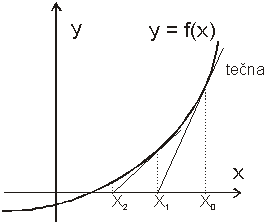
\includegraphics[width=4cm]{matematika/obrazky/newton.png} \end{center}

\begin{reportN}{IOI 21.6.2011} Definujte Tayloruv polynom.
Vyslovte vitu o zbytku Taylorova polynomu.
Vypoetite Taylorovu oadu pro funkci sin(x). 
\end{reportN}
\begin{reportN}{?} fuuuuuuuuuuuuuuuuuuj, dala jsem dohromady zakladni definici, jeden priklad pro exponencialu, jeden priklad zbytku (zkonenej:), pak po me chtel spocitat sin(168 stupnu) pomoc� taylora (coze???), no s velkou pomoci jsem to nejak dala... 
\end{reportN}
\begin{reportN}{Majerech} newtonova metoda (chtel pomoci ni spocitat dom(n)) pricemz Newtona jsem si skoro vubec nepamatoval a smolil a smolil...nakonec jsem delal jen matiku 
\end{reportN}
\begin{reportN}{Matousek} tayloruv polynom, pouziti. A dodal, ze kdybych vedel i nejake tvrzeni, "tak by to bylo skvely" - taylora jsem zadefinoval, napsal i pouziti. Tvrzeni jsem vedel jen jedno jednoduche (nejaka ta limita jde k nule), ale predpoklady moc ne-e - to se mu nelibilo, takze to jeste rozebiral - nejak jsme se dostali ke zbytku a on chtel aspon lagrangeovu vetu o stredni hodnote, ze ktere se to da tak nejak vyjadrit (ja jsem v podstate rekl jen tu vetu, zbytek odrikal on) 
\end{reportN}
\begin{reportN}{nezn�m�} v kazdom pripade newtona si myslim ze spocitas pre nejaky polynom vcelku jednoducho - tak isto ako taylorov polynom pre exp tiez spocitas podla definicie 
\end{reportN}
\begin{reportN}{Majerech} Taylor+zbytek, Newtonova metoda pro funkci x^2+2 a vity o pevn�m bodi. 
Hned na zae�tku mi oekl, �e ty vity o pevn�m bodi co jsme brali nejsou ty, co po mni chce a nadefinoval mi vlastn�, kterou jsem mil dok�zat a nav�c dok�zat, �e neplat� pro fukce nad Q. 
Taylor a NM byly v pohodi, u Taylora staeila definice a NM jsem si pamatoval z numeriky, kdy� jsem se dostal k odm ze dvou s poesnost� na toi m�sta, tak jsme to prohl�sili za konvergentn�. Pak ale zaealo poituhovat. Pou�il jsem metodu nahrazen� kvality kvantitou a sesypal jsem na nikolik A4 �plni v�echna fakta, kter� by se v tom dukazu vity o pevn�m bodi dala pou��t. Pak jsme se v tom dost dlouho poehrabovali a nakonec mi k tomu nijak dokormidloval a kupodivu mi to dal takt� za 1. 
\end{reportN}
\begin{reportN}{Zemlicka} Dalsi otazka bylo hledani korene polynomu numerickymi metodami, tedy Newtonovu metodu + dalsi algoritmy, kde po
me chtel abych srovnal jejich vyhody, nevyhody, rychlosti, ... nicmene musim rict, ze Zemlicka je vic v pohode, nez jsem
cekal. 
\end{reportN}
\begin{reportN}{Klazar} Taylorove polynomu jsem napsala jen, jak vypada, Tayloruv rozvoj funkce, k cemu se to pouziva. Jeste se me pak ptal na par veci, ty uz jsem moc nevedela. A pak jeste rozepsat e na xtou a sin x.  http://forum.matfyz.info/viewtopic.php?f=418&t=3406&p=16319
\end{reportN}

\end{document}
